\section{Experiments}
\label{subsec:results}

\iffalse

\begin{table*}[tb]
    \centering
    \begin{adjustbox}{width=1\columnwidth,center}
		\begin{tabular}{l|l|l|c|c|c|c|c|c|c|c}
			\toprule
			\multirow{3}{0.001\linewidth}{OOD detector} & \multirow{3}{0.10\linewidth}{Hyper-\\parameters} &
			\multirow{3}{0.05\linewidth}{ $\eta^{}_{\bff}(\bfC)$} & \multicolumn{8}{c}{OOD data} \\ \cline{4-11}
    		& & & \multicolumn{2}{c|}{\texttt{Places}} & \multicolumn{2}{c|}{\texttt{SUN}} & \multicolumn{2}{c|}{\texttt{Textures}} & \multicolumn{2}{c}{\texttt{iNaturalist}}\\ \cline{4-11}
    		& & & $\eta^{}_{\bff, S}(\bfC)$ & $J_{\textrm{sep}}(\bfC, \bfC')$ & $\eta^{}_{\bff, S}(\bfC)$ & $J_{\textrm{sep}}(\bfC, \bfC')$ & $\eta^{}_{\bff, S}(\bfC)$ & $J_{\textrm{sep}}(\bfC, \bfC')$ & $\eta^{}_{\bff, S}(\bfC)$ & $J_{\textrm{sep}}(\bfC, \bfC')$ \\ \hline \hline
			\multirow{4}{0.10\linewidth}{MSP \\ \citep{hendrycks2016msp}} 
			& $(0, 0, 0)$ & 0.977 \pm 0.0006 & 0.774 \pm 0.001 & 0.694 \pm 0.0153 & 0.782 \pm 0.001 & 1.088 \pm 0.0175 & 0.593 \pm 0.0013 & 0.765 \pm 0.0157 & 0.878 \pm 0.0008 & 1.075 \pm 0.0191\\
			& $(10, 0.1, 0)$ & \textbf{0.994} \pm 0.0004 & 0.947 \pm 0.0004 & 1.892 \pm 0.0393 & 0.946 \pm 0.0004 & 3.074 \pm 0.0531 & 0.920 \pm 0.0005 & 3.577 \pm 0.1292 & \textbf{0.967} \pm 0.0004 &  \\
			& $(0, 0, 50)$ & 0.980 \pm 0.0005 & 0.814 \pm 0.0008 & 2.533 \pm 0.0714 & 0.816 \pm 0.0009 & 4.295 \pm 0.1048 & 0.773 \pm 0.0010 & 3.147 \pm 0.2076 & 0.864 \pm 0.0007 &\\
			& $(10, 0.1, 50)$ & 0.984 \pm 0.0004 & \textbf{0.960} \pm 0.0004 & 2.756 \pm 0.0854 & \textbf{0.961} \pm 0.0005 & 4.442 \pm 0.0830 & \textbf{0.937} \pm 0.0004 & \textbf{0.439} \pm 0.0175 & 0.946 \pm 0.0004 & \textbf{0.795} \pm 0.0473\\ \hline 
			\multirow{4}{0.10\linewidth}{ODIN \\ \citep{liang2018ODIN}} 
			& $(0, 0, 0)$ & 0.977 \pm 0.0006 & 0.742 \pm 0.0011 & 0.0 & 0.745 \pm 0.0010 & 0.0 & 0.618 \pm 0.0013 & 0.0 & 0.906 \pm 0.0007 & 0.0\\
			& $(\expnum{1}{+8}, 0.1, 0)$ & \textbf{0.994} \pm 0.0004 & 0.951 \pm 0.0004 & -0.118 \pm 0.0099 & 0.958 \pm 0.0004 & -0.054 \pm 0.0119 & 0.934 \pm 0.0004 & -0.245 \pm 0.0133 & 0.935 \pm 0.0004 & -0.345 \pm 0.0153\\
			& $(0, 0, 50)$ & 0.987 \pm 0.0004 & 0.899 \pm 0.0007 & \textbf{0.492} \pm 0.0215 & 0.911 \pm 0.0006 & 0.520 \pm 0.0187 & 0.793 \pm 0.0008 & 0.422 \pm 0.0175 & 0.971 \pm 0.0004 & 0.318 \pm 0.0343\\
			& $(\expnum{1}{8}, 0.1, 50)$ & 0.991 & \textbf{0.973} & 0.355 & \textbf{0.969} & \textbf{0.356} & \textbf{0.945} & 0.405 & \textbf{0.982} & 0.308 \\ \hline
			\multirow{4}{0.10\linewidth}{General-ODIN \\ \citep{hsu2020GeneralizedODIN}} 
			& $(0, 0, 0)$ & 0.990 \pm 0.0004 & 0.869 & 0.0 & 0.869 & 0.0 & 0.850 & 0.0 & 0.981 & 0.0\\
			& $(10^8, 0.1, 0)$ & \textbf{0.994} \pm 0.0004 & 0.951 \pm 0.0006 & 0.161 & 0.959 & 0.215 & 0.936 & 0.411 & 0.936 & 0.151\\
			& $(0, 0, 50)$ & 0.987 & 0.899 & \textbf{0.373} & 0.911 & 0.342 & 0.790 & \textbf{0.414} & 0.970 & \textbf{0.337}\\
			& $(10^8, 0.1, 50)$ & 0.991 & \textbf{0.973} & 0.355 & \textbf{0.969} & \textbf{0.356} & \textbf{0.945} & 0.405 & \textbf{0.982} & 0.308 \\ \hline
			\multirow{4}{0.10\linewidth}{Energy \\ \citep{liu2020energy}} 
			& $(0, 0, 0)$ & 0.977 \pm 0.0006 & 0.671 \pm 0.0012 & 0.0 & 0.682 \pm 0.0012 & 0.0 & 0.557 \pm 0.0014 & 0.0 & 0.871 \pm 0.0007 & 0.0\\
			& $(1. 0.1, 0)$ & \textbf{0.993} \pm 0.0005 & \textbf{0.965} \pm 0.0004 & 0.191 \pm 0.0126 & \textbf{0.963} \pm 0.0004 & 0.326 \pm 0.0133 & \textbf{0.960} \pm 0.0003 & 0.110 \pm 0.0117 & \textbf{0.949} \pm 0.0004 & 0.770 \pm 0.0334\\
			& $(0, 0, 50)$ & 0.987 \pm 0.0005 & 0.779 \pm 0.0010 & 0.4703 \pm 0.0199 & 0.793 \pm 0.0009 & 0.427 \pm 0.0153 &  0.767 \pm 0.0010 & 0.531 \pm 0.0184 & 0.911 \pm 0.0006 & 0.263 \pm 0.0297 \\
			& $(1, 0.1, 50)$ & 0.980 \pm 0.0005 & 0.943 \pm 0.0005 & 0.534 \pm 0.0218 & \textbf{0.941} \pm 0.0005 & 0.534 \pm 0.0175 & 0.936 \pm 0.0005 & 0.658 \pm 0.0212 & 0.927 \pm 0.0005 & 0.291 \pm 0.0319 \\ \hline
			\multirow{4}{0.10\linewidth}{Mahal \\ \citep{lee2018mahalanobis}} 
			& $(0, 0, 0)$ & 0.990 & 0.860 & 0.0 & 0.860 & 0.0 & 0.831 & 0.0 & 0.972 & 0.0 \\
			& $(0.1, 0.1, 0)$ & \textbf{0.994} & 0.962 & 0.153 & 0.963 & 0.176 & 0.962 & 0.351 & 0.955 & 0.169\\
			& $(0, 0, 50)$ & 0.985 & 0.850 & \textbf{0.430} & 0.883 & 0.362 & 0.774 & \textbf{0.429} & 0.926 & \textbf{0.386} \\
			& $(0.1, 0.1, 50)$ & 0.991 & \textbf{0.971} & 0.370 & \textbf{0.970} & \textbf{0.388} & \textbf{0.970} & 0.397 & \textbf{0.972} & 0.351 \\ \bottomrule
		\end{tabular}
	\end{adjustbox}
	\caption[]{\small \textbf{Results of concept learning with different parameter settings across various OOD detectors and OOD datasets.} 
% 	$\bfC'$ denotes a set of concepts discovered by baseline \citep{yeh2020completeness} (\ie $\lambda_\textrm{mse} = 0, \lambda_\textrm{norm} = 0, \lambda_\textrm{sep} = 0$).
	Hyperparameters are in the order of $(\lambda_\textrm{mse}, \lambda_\textrm{norm}, \lambda_\textrm{sep})$. Larger values are better for all the metrics. \textbf{Bold} numbers indicate the best results (across the rows) for a given OOD detection method and dataset. Note that by definition of $J_{\textrm{sep}}(\bfC, \bfC')$ (Eqn. \ref{eq:relative-separability}), the relative concept separability of the baseline~\citep{yeh2020completeness} is always $0$, \ie $J_{\textrm{sep}}(\bfC', \bfC') = 0$.}
	\label{tab:concept-learning-results}
\end{table*}

\fi

\iffalse

We perform experiments to evaluate the proposed method and address the following questions:
\begin{enumerate}[start=1,label={\bfseries Q\arabic*.}]
    \item \label{Q1} Does our concept learning objective effectively encourage concepts to have the desired properties of detection completeness and concept separability?
    \item \label{Q2} Are the proposed evaluation metrics well-aligned with the interpretability of the resulting concept-based explanations?
    % Are the proposed evaluations metrics beneficial for better interpretability of resulting concept-based explanations?
    % \jayaram{Are the proposed evaluation metrics effective at providing better interpretability for the resulting concept-based explanations?}
    % Does a high detection completeness score of concepts imply a more accurate explanaation of the OOD detector? Does better concept separability lead to a more distinctive explanation between ID- and OOD-detected data?
    \item \label{Q3} Given concepts learned by our approach, what insights can we provide for the OOD detector?
\end{enumerate}

Our main findings are summarized as follows:
\begin{enumerate}[start=1,label={\bfseries A\arabic*.}]
    \item In accordance with our design intention, our $\ell_2$ norm-based regularization and MSE regularization not only improve the detection completeness by large margin, but also the classification completeness even further. 
    The proposed separability regularization effectively improves concept separability, and when these three terms are used together in concept learning objective, we can achieve the highest detection completeness and concept separability (see Table \ref{tab:concept-learning-results}).
    \item Concepts with a high completeness score enable to mimic the original behavior of the OOD detector more precisely, hence leading to more \textit{accurate} explanations based on the concepts (see Fig. \ref{fig:score-distribution}). 
    Also, concepts with a higher concept separability score lead to more \textit{visually-distinctive} interpretations between ID and OOD data by having more distinguishable concept-score patterns (see Fig. \ref{fig:high_separa_interpretatbility}).
    % Concepts learned by our method enable more \textit{accurate}, and more \textit{visually distinctive} interpretations, compared to the concepts learned by the baseline method (\citep{yeh2020completeness}).
    \item We can rank the importance of each concept towards OOD detection using the Shapley value modified with our per-class detection completeness metric. 
    When the concepts are only targeted at explaining the DNN classifier (as in the baseline \citep{yeh2020completeness}), the behavior of the OOD detector is merely described by the common set of concepts that are important for the DNN classifier.
    On the other hand, when not only the DNN classifier but also the OOD detector is taken into consideration during concept learning (\ie our method), we obtain a more diverse and expanded set of concepts, and different concepts play a major role in interpreting the classification and detection results (see Fig. \ref{fig:shap_buffalo}). 
    % identify based on what concepts an OOD detector makes decisions.
    % We can identify the top concepts that contribute to the OOD detector's decisions using  
\end{enumerate}



\fi

In this section, we conduct experiments to evaluate the proposed method and show that: 1) the learned concepts satisfy the desiderata of completeness and separability across popular off-the-shelf OOD detectors and real-world datasets. 2) the learned concepts can be combined with a Shapley value to provide insightful visual explanations that can help understand the predictions of an OOD detector. 
The code for our work can be found at \url{https://github.com/jihyechoi77/concepts-for-ood}.
% In this section, we conduct experiments to show that our method can learn concepts that satisfy the desiderata of completeness and separability across popular off-the-shelf OOD detectors and real-world datasets.
% We start the experimental section by answering the fundamental question: \textit{can our concept learning framework find a good set of concepts that satisfy the desiderata of completeness and separability as intended?}
% We observe that the resulting concepts have high completeness and separability scores when evaluated with real-world ID and OOD images, and targeted for popular off-the-shelf OOD detectors.

\subsection{Experimental Setup}
\label{sec:setup}
% We briefly describe the experimental setup here and provide additional details in Appendix \ref{sec:appendix-implementation-details}.
% We briefly describe the setup of our experiments to address the above questions. See Appendix \ref{sec:appendix-implementation-details} for further details.
% For reproducibility, we have released our anonymized source code ~\footnote{\url{https://anonymous.4open.science/r/Concept-For-OOD-CE1B/}}.

\mypara{Datasets.} For the ID dataset, we use Animals with Attributes (AwA) \citep{xian2018awa} with 50 animal classes, and split it into a train set (29841 images), validation set (3709 images), and test set (3772 images).
We use the MSCOCO dataset \citep{lin2014mscoco} as the auxiliary OOD dataset $\Douttr$ for training and validation.
For the OOD test dataset $\Doutte$, we follow the literature of large-scale OOD detection \citep{Huang_MOS} and use three different image datasets: \texttt{Places365} \citep{zhou2017places}, \texttt{SUN} \citep{xiao2010sun}, and \texttt{Textures} \citep{cimpoi2014textures}.
% , \texttt{iNaturalist} \citep{van2018inaturalist}; all resized to the input size $224 \times 224$.

% \textbf{OOD detector.} We apply our general approach to intepret four popular OOD detection methods in the literature: MSP \citep{hendrycks2016msp}, ODIN \citep{liang2018ODIN}, Energy \citep{liu2020energy} and Mahalanobis \citep{lee2018mahalanobis} (henceforth abbreviated to Mahal).

% \jihye{real-world high resolution image data}
% \textbf{DNN classifier.} The OOD detectors are paired with the widely-used Inception-V3 model \citep{szegedy2016inception-v3} (following the common setup in prior works \citep{yeh2020completeness, ghorbani2019ace, koh2020concept-bottleneck, kim2018tcav}) trained on AwA, which yields $0.921$ test accuracy. 


\mypara{Models.}
We apply our framework to interpret five prominent OOD detectors from the literature: MSP~\citep{hendrycks2016msp}, ODIN~\citep{liang2018ODIN}, Generalized-ODIN~\citep{hsu2020GeneralizedODIN}, Energy~\citep{liu2020energy}, and Mahalanobis~\citep{lee2018mahalanobis}.
The OOD detectors are paired with the widely-used Inception-V3 classifier~\citep{szegedy2016inception-v3} (following the setup in prior works~\citep{yeh2020completeness, ghorbani2019ace, kim2018tcav}), which has a test accuracy of $92.13 \%$ on the AwA dataset.
% trained on the Animals-with-Attributes (AwA) dataset~\citep{xian2018awa}, . 
% \subsection{Results}\label{subsec:results}
%
Additional details on the setup are given in Appendix~\ref{sec:appendix-implementation-details}.
% Codes for reproducibility are submitted as supplementary material.
 
\subsection{Effectiveness of the Concept Learning}
\label{sec:eval-concept}
% In this subsection, we elaborate on the experiments to answer the first question (Q1) on the effectiveness of our concept learning objective.
Table~\ref{tab:concept-learning-results-places} summarizes the results of concept learning for various combinations of the regularization coefficients ($\lambda_{\star}$) in Eqn (\ref{equ: concept learning}), including: \textbf{i)} baseline where all the coefficients are set to $0$ (first row); \textbf{ii)} only the terms directly relevant to detection completeness (\ie $J_{\textrm{norm}}(\bfC, \bfg)$ and $J_{\textrm{mse}}(\bfC, \bfg)$) are included (second row); \textbf{iii)} only the term responsible for concept separability $J_{\textrm{sep}}(\bfC)$ is included (third row); \textbf{iv)} all the regularization terms are included (fourth row).

From the table, we observe that the regularization terms encourage the learned concepts to satisfy the required desiderata of high completeness and concept separability scores.
% Given any OOD detector, we confirm the design of regularization terms to encourage the desiderata of concepts.
Having $\lambda_\textrm{mse} > 0\, \text{ and } \,\lambda_\textrm{norm} > 0$ always improves the detection completeness by a large margin (\ie row 2 compared to row 1), and having $\lambda_\textrm{sep} > 0$ significantly increases the concept separability (\ie row 3 compared to row 1).
% In accordance with our design intention, our $\ell_2$ norm-based regularization and MSE regularization not only improve the detection completeness by large margin, but also the classification completeness even further.
Importantly, when all the regularization terms are included, they have the best synergistic effect on the metrics. 
% More importantly, the three terms make the best synergy together in most cases.

\begin{table}[thb]
    \centering
    \begin{adjustbox}{width=1\columnwidth,center}
    % \begin{adjustbox}{width=1\textwidth,center}
		\begin{tabular}{l|l|c|c|c}
			\toprule
			OOD detector & $(\lambda_\textrm{mse}, \lambda_\textrm{norm}, \lambda_\textrm{sep})$ &
			$\eta^{}_{\bff}(\bfC) \uparrow$ & $\eta^{}_{\bff, S}(\bfC) \uparrow$ & $J_{\textrm{sep}}(\bfC, \bfC') \uparrow$ \\ \hline \hline
            \multirow{4}{0.10\linewidth}{MSP} 
			& $(0, 0, 0)$ & 0.977 $\pm$ 0.0006 & 0.774 $\pm$ 0.0010 & 0.694 $\pm$ 0.0153 \\
			& $(10, 0.1, 0)$ & \textbf{0.994} $\pm$ 0.0004 & \underline{0.947} $\pm$ 0.0004 & 1.892 $\pm$ 0.0393 \\
			& $(0, 0, 50)$ & 0.980 $\pm$ 0.0005 & 0.814 $\pm$ 0.0008 & \underline{2.533} $\pm$ 0.0714 \\
			& $(10, 0.1, 50)$ & \underline{0.984} $\pm$ 0.0004 & \textbf{0.960} $\pm$ 0.0004 & \textbf{2.756} $\pm$ 0.0854 \\ \hline
			%
            \multirow{4}{0.10\linewidth}{ODIN} 
			& $(0, 0, 0)$ & 0.977 $\pm$ 0.0006 & 0.742 $\pm$ 0.0011 & 0.444 $\pm$ 0.0119 \\
			& $(10^8, 0.1, 0)$ & \textbf{0.994} $\pm$ 0.0004 & \underline{0.951} $\pm$ 0.0004 & 1.166 $\pm$ 0.0303 \\
			& $(0, 0, 50)$ & 0.987 $\pm$ 0.0004 & 0.899 $\pm$ 0.0007 & \underline{1.785} $\pm$ 0.0669 \\
			& $(10^8, 0.1, 50)$ & \underline{0.991} $\pm$ 0,0005 & \textbf{0.973} $\pm$ 0.0009 & \textbf{1.813} $\pm$ 0.0268 \\ \hline
			%
            \multirow{4}{0.10\linewidth}{General-ODIN} 
			& $(0, 0, 0)$ & 0.988 $\pm$ 0.0004 & 0.769 $\pm$ 0.0004 & 0.506 $\pm$ 0.0165 \\
			& $(10^6, 0.1, 0)$ & \textbf{0.995} $\pm$ 0.0004 & \underline{0.951} $\pm$ 0.0006 & 1.461 $\pm$ 0.0321 \\
			& $(0, 0, 50)$ & 0.981 $\pm$ 0.0004 & 0.859 $\pm$ 0.0007 & \underline{1.814} $\pm$ 0.0685 \\
			& $(10^6, 0.1, 50)$ & \underline{0.990} $\pm$ 0.0005 & \textbf{0.971} $\pm$ 0.0010 & \textbf{1.835} $\pm$ 0.0669 \\ \hline
			%
            \multirow{4}{0.10\linewidth}{Energy} 
			& $(0, 0, 0)$ & 0.977 $\pm$ 0.0006 & 0.671 $\pm$ 0.0012 & 0.453 $\pm$ 0.0121 \\
			& $(1. 0.1, 0)$ & \textbf{0.993} $\pm$ 0.0005 & \textbf{0.965} $\pm$ 0.0004 & 1.266 $\pm$ 0.0319 \\
			& $(0, 0, 50)$ & \underline{0.987} $\pm$ 0.0005 & 0.779 $\pm$ 0.0010 & \textbf{1.920} $\pm$ 0.0725 \\
			& $(1, 0.1, 50)$ & 0.980 $\pm$ 0.0005 & \underline{0.943} $\pm$ 0.0005 & \underline{1.839} $\pm$ 0.0662 \\ \hline
			%
			\multirow{4}{0.10\linewidth}{Mahalanobis} 
			& $(0, 0, 0)$ & 0.990 $\pm$ 0.0007 & 0.715 $\pm$ 0.0011 & 0.571 $\pm$ 0.0110 \\
			& $(0.1, 0.1, 0)$ & \textbf{0.994} $\pm$ 0.0004 & \underline{0.950} $\pm$ 0.0009 & 1.532 $\pm$ 0.0351 \\
			& $(0, 0, 50)$ & 0.985 $\pm$ 0.0004 & 0.880 $\pm$ 0.0005 & \underline{2.550} $\pm$ 0.0681 \\
			& $(0.1, 0.1, 50)$ & \underline{0.992} $\pm$ 0.0006 & \textbf{0.961} $\pm$ 0.0005 & \textbf{2.616} $\pm$ 0.0857 \\ \bottomrule
		\end{tabular}
	\end{adjustbox}
	\caption[]{
	\small Concept learning results with different parameter settings across various OOD detectors, evaluated on AwA test set (ID) and \texttt{Places365} (OOD). 
% 	$\bfC'$ denotes a set of concepts discovered by baseline \citep{yeh2020completeness} (\ie $\lambda_\textrm{mse} = 0, \lambda_\textrm{norm} = 0, \lambda_\textrm{sep} = 0$).
% 	Larger values are better for all the metrics. 
Hyperparameters are set based on the scale of corresponding regularization terms for a specific choice of the OOD detector.
 Across the rows (for a given OOD detector), the best value is \textbf{boldfaced}, and the second best value is \underline{underlined}.
	The $95\%$ confidence intervals are estimated by bootstrapping the test set over $200$ trials. Complete results are given in Table~\ref{tab:concept-learning-results} in Appendix~\ref{sec:app_addi_results}.
% 	\textbf{Bold} numbers indicate the best results (across the rows) for a given OOD detection method and dataset. 
	%Note that by definition of $J_{\textrm{sep}}(\bfC, \bfC')$ (Eqn. \ref{eq:relative-separability}), the relative concept separability of the baseline~\citep{yeh2020completeness} is always $0$, \ie $J_{\textrm{sep}}(\bfC', \bfC') = 0$.
	}
\label{tab:concept-learning-results-places}
% \vspace{-.5in}
\end{table}
%


%\jihye{@Jayaram: not sure if mentioning this instance is necessary. } 
Consider the MSP detector for instance. The detection completeness increases from $0.774$ to $0.947$ with $\lambda_\textrm{mse} = 10, \lambda_\textrm{norm} = 0.1, \lambda_\textrm{sep} = 0$, and the concept separability increases from $0.694$ to $2.533$ with $\lambda_\textrm{mse} = 0, \lambda_\textrm{norm} = 0, \lambda_\textrm{sep} = 50$.
However, when all the terms are considered ($\lambda_\textrm{mse} = 10, \lambda_\textrm{norm} = 0.1, \lambda_\textrm{sep} = 50$), we achieve the best result of $\eta^{}_{\bff, S}(\bfC) = 0.960$ and $J_{\textrm{sep}}(\bfC, \bfC') = 2.756$. 
Results on other large-scale OOD datasets and ablation studies on the regularization terms can be found in Appendix \ref{sec:appendix-concept-learning-ablation}.

\iffalse

% \mypara{Metrics.}
% For each set of concepts learned with different OOD detectors and hyperparameters, we report the classification completeness $\eta^{}_{\bff}(\bfC)$, detection completeness $\eta^{}_{\bff, S}(\bfC)$, and the relative concept separability metric (defined below). 
In contrast to the completeness scores (\ie $\eta^{}_{\bff}(\bfC)$ and $\eta^{}_{\bff, S}(\bfC)$) that are almost always bounded to the range $[0, 1]$, it is hard to gauge the possible range of the separability score $J_{\textrm{sep}}(\bfC)$ (or $J^y_{\textrm{sep}}(\bfC)$) across different settings (datasets, classification models, and OOD detectors), and whether the value represents a significant improvement in separability.
Hence, in Table~\ref{tab:concept-learning-results-places}, we define and report the \textit{relative concept separability}, which captures the relative improvement in concept separability using concepts $\bfC$ compared to a different set of concepts $\bfC'$, as follows
% between two different sets of concepts, as follows
% \vspace{-1mm}
\begin{equation}
\label{eq:relative-separability}
J_{\textrm{sep}}(\bfC, \bfC') = \textrm{Median}\left( \left\{\frac{J^y_{\textrm{sep}}(\bfC) ~-~ J^y_{\textrm{sep}}(\bfC')}{J^y_{\textrm{sep}}(\bfC')}\right\}_{y=1}^L \right). 
\end{equation}
% This metric measures the median of the relative increase in the per-class separability using concepts $\bfC$, compared to that of using a different set of concepts $\bfC'$.
where $\bfC'$ is fixed as the set of concepts learned by the baseline of $\,\lambda_\textrm{mse} = \lambda_\textrm{norm} = \lambda_\textrm{sep} = 0$.
% The set of concept $\bfC$ is obtained via our concept learning objective, with various combinations of hyperparameter values.

\fi

Since the range of the separability score $J_{\textrm{sep}}(\bfC)$ (or $J^y_{\textrm{sep}}(\bfC)$) is not well defined, we report a \textit{relative concept separability} score that is easier to interpret, and defined as
\begin{equation}
\label{eq:relative-separability}
J_{\textrm{sep}}(\bfC, \bfC') = \textrm{Median}\left( \left\{\frac{J^y_{\textrm{sep}}(\bfC) ~-~ J^y_{\textrm{sep}}(\bfC')}{J^y_{\textrm{sep}}(\bfC')}\right\}_{y=1}^L \right). 
\end{equation}
It captures the relative improvement in concept separability using concepts $\bfC$, compared to a baseline set of concepts $\bfC'$ obtained by setting $\,\lambda_\textrm{mse} = \lambda_\textrm{norm} = \lambda_\textrm{sep} = 0$.
%

% We test how effectively our regularization terms improve detection completeness and concept separability, without sacrificing the classification completeness.
\mypara{Concepts good for the OOD detector are also good for the classifier, but not vice-versa.} 
Recall that the baseline $(\lambda_\textrm{mse} = \lambda_\textrm{norm} = \lambda_\textrm{sep} = 0)$ corresponds to the method of \citet{yeh2020completeness} where only the classifier is considered during the concept learning.
For any choice of OOD detector in Table~\ref{tab:concept-learning-results-places} and Table~\ref{tab:concept-learning-results} (in Appendix~\ref{sec:app_addi_results}), the concepts learned by our method always achieve higher scores even for classification completeness, compared to the baseline. 
In contrast, the baseline concepts for only the classifier have the lowest detection completeness and concept separability in all cases.
This may not be surprising since the scope of~\citet{yeh2020completeness} does not cover explaining detectors.
%Nonetheless, such observations become the supporting evidence of our motivation for this paper,
Nonetheless, such observations provide supporting evidence to motivate the need for our concept learning and novel metrics, indicating that {\em even if the concepts are sufficient to describe the DNN classifier, the same set of concepts may not be appropriate for the OOD detector.}

% We also observe that concept separability regularization term $J_{\textrm{sep}}(\bfC) > 0$ improves the relative concept separability, and when brought together with $J_{\textrm{norm}}(\bfC, \bfg)$ and  $J_{\textrm{mse}}(\bfC, \bfg) = 0$, can improve the detection completeness even further.
% By having $\lambda_\textrm{mse} > 0, \lambda_\textrm{norm} > 0, \lambda_\textrm{sep} = 0$, we observe that $\eta^{}_{\bff, S}(\bfC)$ is always improved by large margin compared to baseline.
%
% We observe that the relative concept separability $J_{\textrm{sep}}(\bfC, \bfC')$ is largest most often for the setting where $\lambda_\textrm{mse} = \lambda_\textrm{norm} = 0, \text{ and } \lambda_\textrm{sep} > 0$ (third row).
% However, the detection completeness does not improve and in some cases drops compared to the baseline setting, suggesting that there is a tradeoff between maximizing the detection completeness and concept separability.
%

% \jihye{For instance, given the ODIN detector and the \texttt{SUN} dataset, including our proposed regularization terms improves the detection completeness of concepts from $0.869$ to $0.969$, and the relative concept separability is increased by $0.356$, compared to when concepts are learned without the regularization terms.}
% In this setting, there is a slight decrease the relative concept separability compared to the case where only the regularization term $J_{\textrm{sep}}(\bfC)$ is included (third row). In other words, there is a tradeoff wherein we may have to sacrifice the concept separability a little in order to achieve the best possible detection completeness.


\iffalse
\mypara{Choice of Hyperparameters.}
\label{sec:hyperparameter}
In Table \ref{tab:concept-learning-results}, we set the values of $\lambda_{\textrm{norm}}, \lambda_{\textrm{mse}}$ and $\lambda_{\textrm{sep}}$ based on the scale of corresponding regularization terms in Eqn. (\ref{equ: concept learning}) (\ie $J_{\textrm{norm}}(\bfC, \bfg),  J_{\textrm{mse}}(\bfC, \bfg)$ and $ J_{\textrm{sep}}(\bfC)$, respectively) for a specific choice of the OOD detector.
Further investigation including an ablation study on each regularization term can be found in Appendix \ref{sec:appendix-concept-learning-ablation}.
From the ablation study, we note that there is a trade-off between concept separability and coherency (defined in Eqn. \ref{eq:coherency}).
This implies that high concept separability ensures easily distinguishable score patterns between detected-ID and detected-OOD inputs, but the discovered concepts may not be understandable to humans, hence the user needs to balance the degree of $\lambda_{\textrm{sep}}$ depending on the application of interest. 
\fi
% Interestingly, we observe that the concepts targeted for a particular type of OOD detector can also be applied to different types of OOD detectors (\ie the learned concepts exhibit transferability). 
% Transferability of concepts across different OOD detectors is also discussed in Appendix \ref{sec:appendix-concept-learning-transfer}.
\iffalse
\begin{figure}[h]
\centering
\subfigure{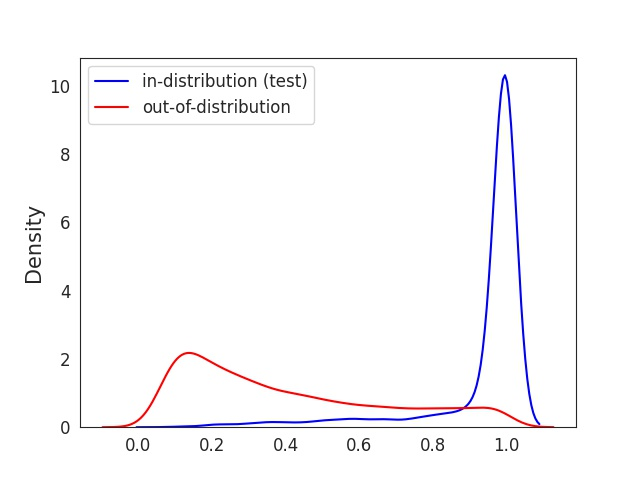
\includegraphics[width=0.31\textwidth]{figures/distr_msp_target.jpg}} 
\subfigure{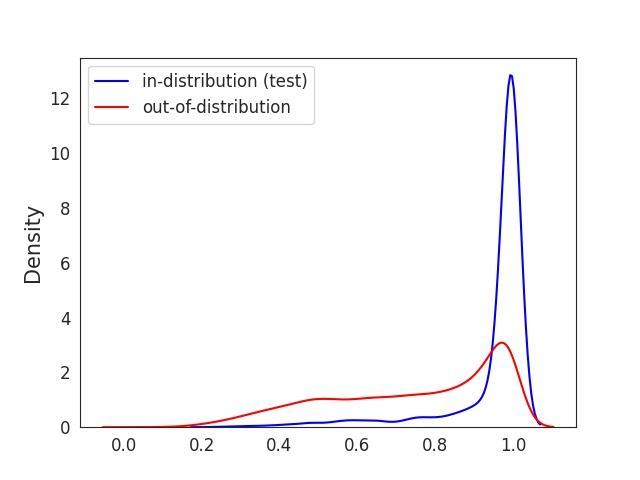
\includegraphics[width=0.31\textwidth]{figures/distr_msp_yeh.jpg}} 
\subfigure{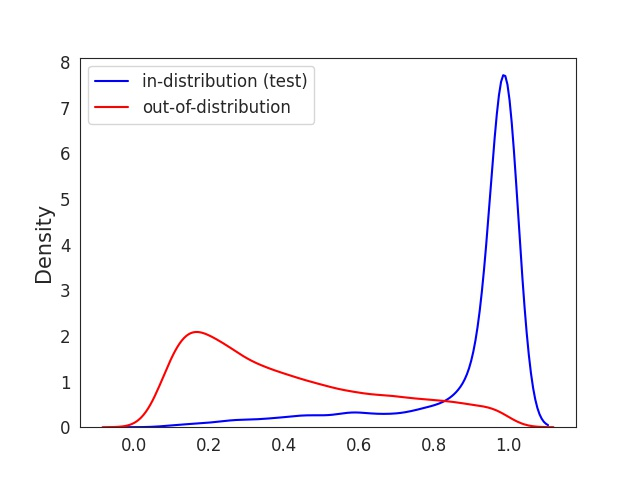
\includegraphics[width=0.31\textwidth]{figures/distr_msp_ours.jpg}} 
\caption{\textbf{Detection completeness and estimated density of OOD score $S(\bfx, \bff)$ from MSP detector.}
\textbf{Left}: Target distribution of $S(\bfx, \bff)$ in the canonical world. 
\textbf{Mid}: Distribution of $\Scon(\bfx, \bff)$ in the concept world, using concepts learned by \citep{yeh2020completeness} ($\,\lambda_\textrm{mse} = \lambda_\textrm{norm} = \lambda_\textrm{sep} = 0$).
\textbf{Right}: Distribution of $\Scon(\bfx, \bff)$ in the concept world, using concepts learned by our method ($\lambda_\textrm{mse} = 10, \lambda_\textrm{norm} = 0.1, \lambda_\textrm{sep} = 50$). Comparison is made between AwA test set (ID; blue) vs. SUN (OOD; red).}
\label{fig:score-distribution-msp}
\end{figure}
\fi

\begin{figure*}[hbt]
% \vspace{-5mm}
     
     \begin{subfigure}[b]{0.7\textwidth}
     \centering
     \begin{subfigure}{\textwidth}
         \centering
         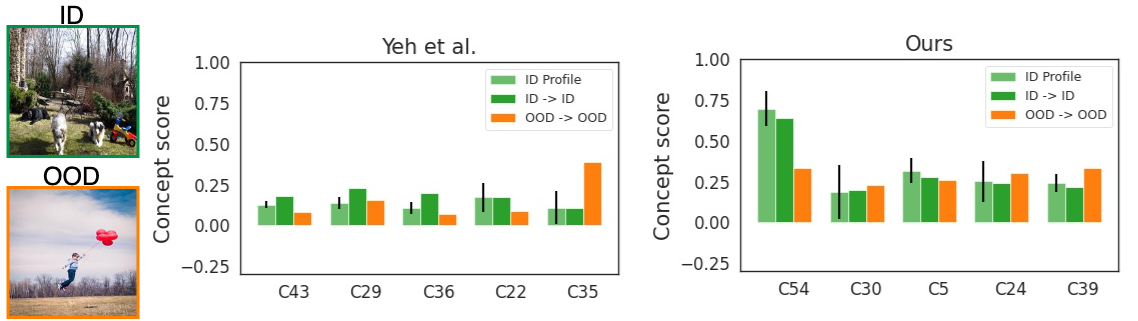
\includegraphics[width=\textwidth]{figures/fig3a.png}
         \caption{\small Correct detection: top collie image is correctly detected as ID (dark-green bar), and the bottom image is correctly detected as OOD (orange bar).}
         % ID (or OOD) dolphin image correctly detected as ID (or OOD).
         \label{fig:collie-correct}
     \end{subfigure}
     \\
     \begin{subfigure}{\textwidth}
         \centering
         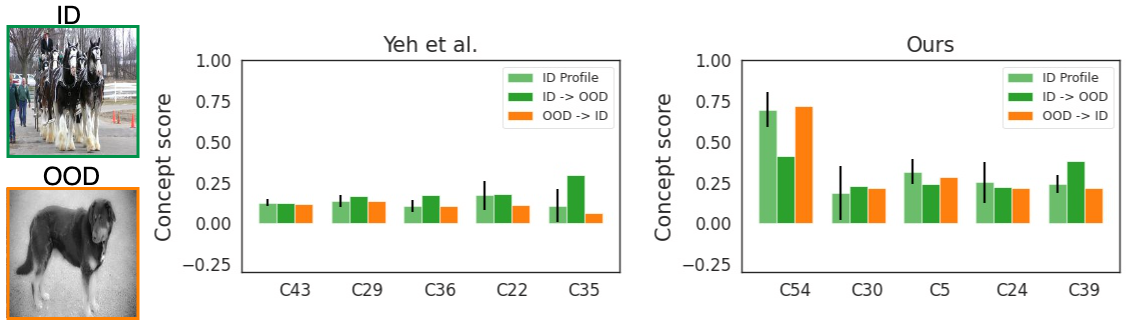
\includegraphics[width=\textwidth]{figures/fig3b.png}
         \caption{\small Wrong detection: top ID image is detected as OOD (dark-green bar), and the bottom OOD image is detected as ID (orange bar).}
         % ID (or OOD) dolphin image falsely detected as OOD (or ID).
         \label{fig:collie-wrong}
     \end{subfigure}
     \end{subfigure}
     \hspace{2mm}
     \begin{subfigure}[b]{0.23\textwidth}
         \centering
         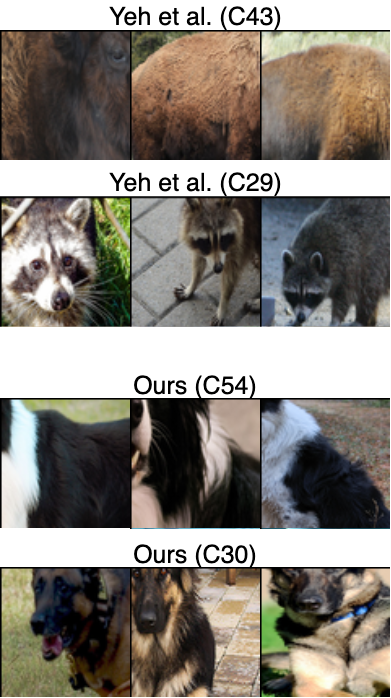
\includegraphics[width=\textwidth]{figures/fig3c.png}
         \caption{\small Visualization of top-2 important concepts found by the method of \citet{yeh2020completeness} and our method.}
         \label{fig:collie-concepts}
     \end{subfigure}
% \begin{subfigure}[b]{0.3\textwidth}
%     \centering
%     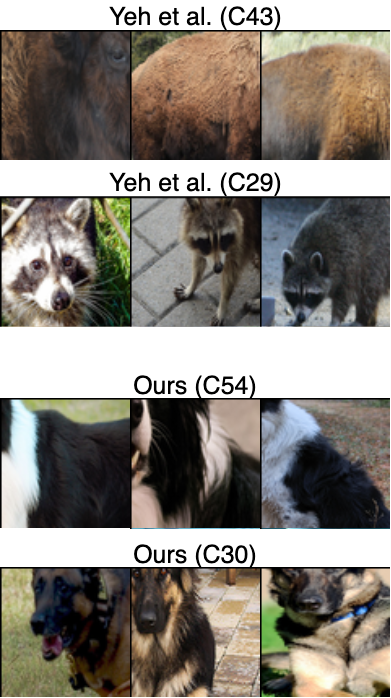
\includegraphics[width=0.9\textwidth]{figures/fig3c.png}
% \end{subfigure}
\caption{\small \textbf{Concept-based explanations for the Energy OOD detector using concepts learned by \citet{yeh2020completeness} vs. ours ($\lambda_\textrm{mse} = 1, \lambda_\textrm{norm} = 0.1, \lambda_\textrm{sep} = 10$)}. Images are randomly selected from the AwA test set (ID) and \texttt{Places} (OOD), and all of them are predicted to the class ``Collie''. Concept score patterns by \citet{yeh2020completeness} are not distinctive between detected-ID vs. detected-OOD (\ie dark-green bar and orange bar are not very different). Whereas, our concepts present very similar patterns to the ID profile (light-green bar) when input is detected as ID, and different from the ID profile when detected as OOD.
}
\label{fig:expl-energy-collie}

\end{figure*}




% \subsection{Interpretability of the Learned Concepts (Q2.)}
% \subsection{Our Metrics and Interpretability (Q2.).}
% \mypara{Reconstruction of $\hat{\calZ}$.}

% \mypara{Detection completeness and accurate reconstruction of $\calZ$.}
\mypara{Accurate Reconstruction of Per-sample Behavior.}
% Other than observing increased detection completeness, 
% To gain further insights on how accurately the feature representation space can be reconstructed from concept scores, 
% Fig. \ref{fig:score-distribution} compares the distribution of the OOD detector scores in the canonical world and concept world using the concepts with different level of detection completeness.
% learned by baseline and ours. 
% Taking MSP and Energy detectors as example, 
% Additionally, we observe whether the proposed evaluation metrics are well-aligned with the interpretability of the resulting concept-based explanations.
In addition to the above numerical comparisons with respect to the proposed metrics, we found the method of \citet{yeh2020completeness} to have potential issues in terms of reconstructing the feature representations. This in-turn leads to degraded reconstruction of the \textit{per-sample} behavior of the OOD detector.
Comparing Fig.~\ref{fig:short-a} and Fig.~\ref{fig:short-b}, we observe that the concepts of \citet{yeh2020completeness} lead to a strong mismatch between the score distributions of the OOD detector. In contrast, our method approximates the score distributions more closely (compare Fig.~\ref{fig:short-a} and Fig.~\ref{fig:short-c}).
% In Fig.~\ref{fig:short-a} vs. Fig.~\ref{fig:short-b}, concepts by ~\citep{yeh2020completeness} lead to a strong mismatch between the score distributions, while ours approximate the target score distributions more closely (see Fig.~\ref{fig:short-a} vs. Fig.~\ref{fig:short-c}).
Given that the second half of the classifier and detector remains fixed between the canonical and concept worlds, this observation implies that the reconstructed features fed into the second half of the classifier have to be distorted. Similar observations are made for the Energy detector in Fig.~\ref{fig:score-distribution-energy} in Appendix~\ref{sec:app_addi_results}.
% Overall, our experiments find that the proposed regularization terms reduce the performance gap (between the canonical world and concept world) of both the classifier and the OOD detector, leading to more \textit{accurate} explanations.
% This validates our hypothesis that accurate reconstruction of the feature representation space $\hat{\calZ}$ and the score functions are both crucial for closing the performance gap between the canonical world and concept world of both the classifier and the OOD detector.
% By reducing the performance gap of OOD detector between canonical world and concept world, it leads to more \textit{accurate} explanations for OOD detectors.
% \begin{tcolorbox}
% {\textbf{Takeaway}: Our proposed concept learning objective can achieve high detection completeness and concept separability given various OOD detectors. By reducing the performance gap of OOD detector between canonical world and concept world, it leads to more \textit{accurate} explanations for OOD detectors.} 
% \end{tcolorbox}
% even though the classification completeness is quite high, the distribution of reconstructed scores from the OOD detector 
%  is significantly different from the original distribution of scores in the canonical world 
We observe that such inaccurate reconstruction of features poses a similar problem for classifiers as well (more discussion in Appendix~\ref{app:hellinger}).
We conclude that the objective of \citet{yeh2020completeness}, which considers only the aggregate statistic of reconstructed accuracy, is not sufficient to recover the per-sample behavior, and augmenting it with our reconstruction error-based regularization term is a straightforward improvement for both the classifier and OOD detector.
% Accordingly, our concepts lead to a more accurate approximation of the per-sample classifier predictions, which in turn enables more accurate interpretation of both the OOD detector and the classifier.

 
\iffalse

\begin{figure}[bt]
\centering
\subfloat[Set 1 with low concept separability, detected-ID \label{fig:low_in}]{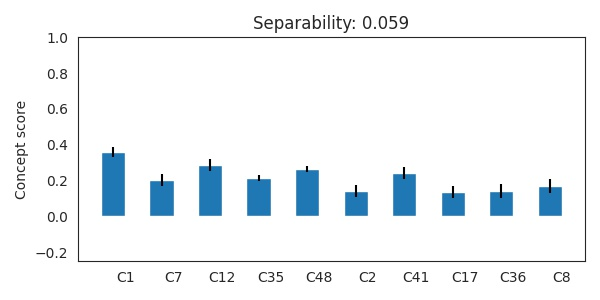
\includegraphics[width=0.45\columnwidth]{yeh_class17_AwA2_top10_detected_Energy.jpg}}
\hfill \hspace{-2mm}
\subfloat[Set 2 with high concept separability, detected-ID \label{fig:high_in}] {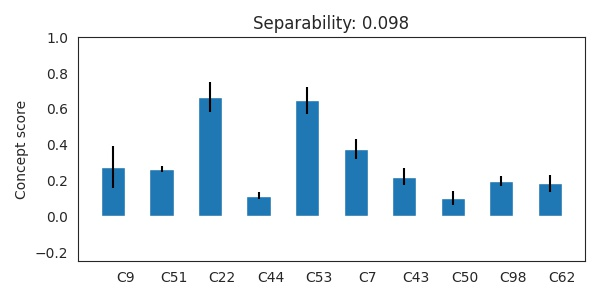
\includegraphics[width=0.45\columnwidth]{figures/ours_class17_AwA2_top10_detected_Energy.jpg}}\hfill\\
% \vspace{-1mm}
\subfloat[Set 1 with low concept separability, detected-OOD \label{fig:low_out}]{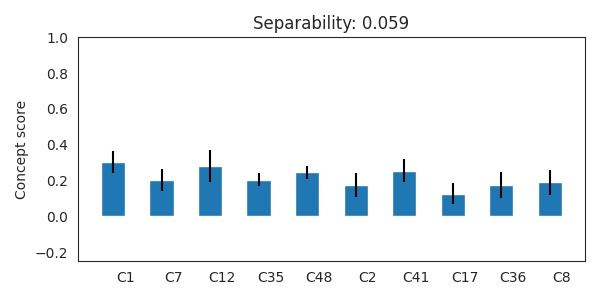
\includegraphics[width=0.45\columnwidth]{figures/yeh_class17_SUN_top10_detected_Energy.jpg}}\hfill
\subfloat[Set 2 with high concept separability, detected-OOD \label{fig:high_out}] {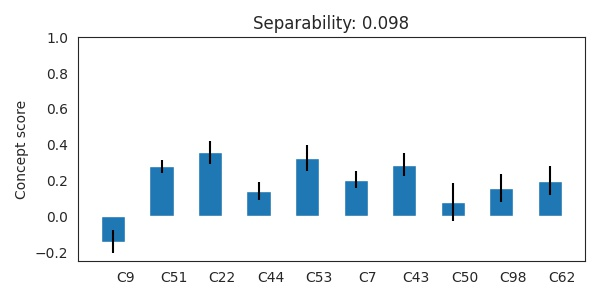
\includegraphics[width=0.45\columnwidth]{figures/ours_class17_SUN_top10_detected_Energy.jpg}}
\caption{
\small \textbf{Our concept separability metric and visual distinction in the concept score patterns.} For the class "Giraffe", we compare the concept score patterns using two different sets of concepts. \textbf{Left:} Averaged concept scores using concept set 1 (top-10 important concepts out of the concepts learned with $\,\lambda_\textrm{mse} = \lambda_\textrm{norm} = \lambda_\textrm{sep} = 0$). 
\textbf{Right:} Averaged concept scores using concept set 2 (top-10 important concepts out of the concepts learned with $\,\lambda_\textrm{mse} = 1, \lambda_\textrm{norm} = 0.1, \lambda_\textrm{sep} = 50$).
Concept importance is measured using the Shapley value of Eqn. (\ref{equ: ConceptSHAP}).
Concept separability is measured based on the presented 10 concepts from each set.
% For visualization of what each concept represents, see Appendix.
% C$i$ denotes $i$-th concept.
}
\label{fig:high_separa_interpretatbility}
\vspace{-0.10in}
% \vspace{-4mm}
\end{figure}

\fi

% Lastly, we illustrate how the concepts learned by our algorithm can be used to provide explanations for an OOD detector.
% By quantifying the contribution of each concept toward OOD detection results, we can identify the major concepts that an OOD detector relies on to make decisions. 
% \begin{itemize}
%     \item What set of the concepts is most prominent across the data detected as ID (or OOD) by $\mathcal{D}$?
%     \item What set of the concepts contribute to distinguish the ID and OOD data detected by $\mathcal{D}$?
%     \item How the change in concept score affects the $\mathcal{D}$'s detection result?
%     % \jihye{check perturbation generation in ATOM <-- permutation in concept space?}
% \end{itemize}
%

\iffalse

\begin{figure}[tb]
\vspace{-5mm}
% \begin{center}
%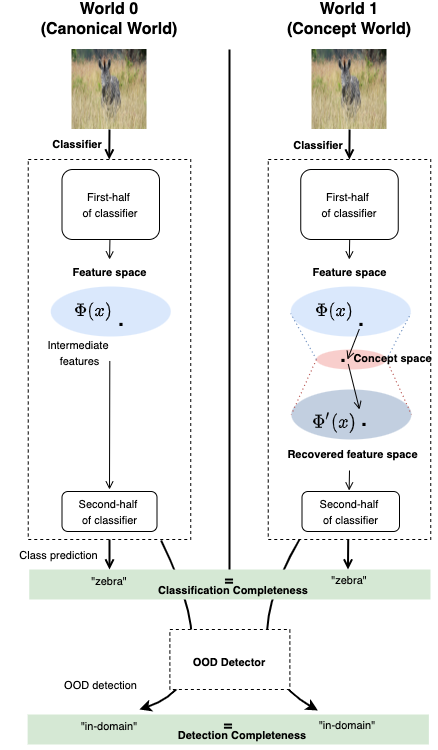
\includegraphics[width=0.45\textwidth]{figures/completeness.png}
% \hspace*{+.5cm} 
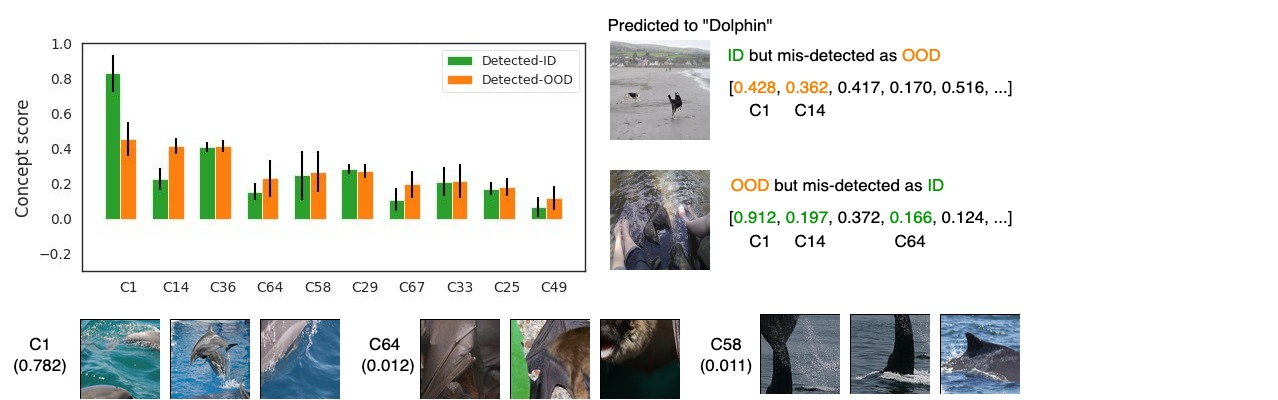
\includegraphics[scale=0.35]{figures/expl_dolphin.png}
% \vspace{-9mm}
\caption{
\small \textbf{Our concept-based explanations for Energy detector given AwA (ID) and SUN (OOD) inputs.} Concepts are discovered by our method with $\lambda_\textrm{mse} = 1, \lambda_\textrm{norm} = 0.1, \lambda_\textrm{sep} = 10$.
Visualized examples for each concept (with the corresponding $\textrm{SHAP}(\eta^{j}_{\bff, S}, 
    \bfc_i)$ score inside the parenthesis) are the receptive fields from $\Dinte$ with highest correlation to the corresponding concept vector $\bfc_i$ where $\langle \bfphi^{p,q}(\bfx), \bfc_i \rangle > 0.85$.
\vspace{-5mm}
}
\label{fig:expl_dolphin}
% \end{center}
\end{figure}

\fi

\iffalse
\begin{figure*}[t]
% \vspace{-3mm}
\centering
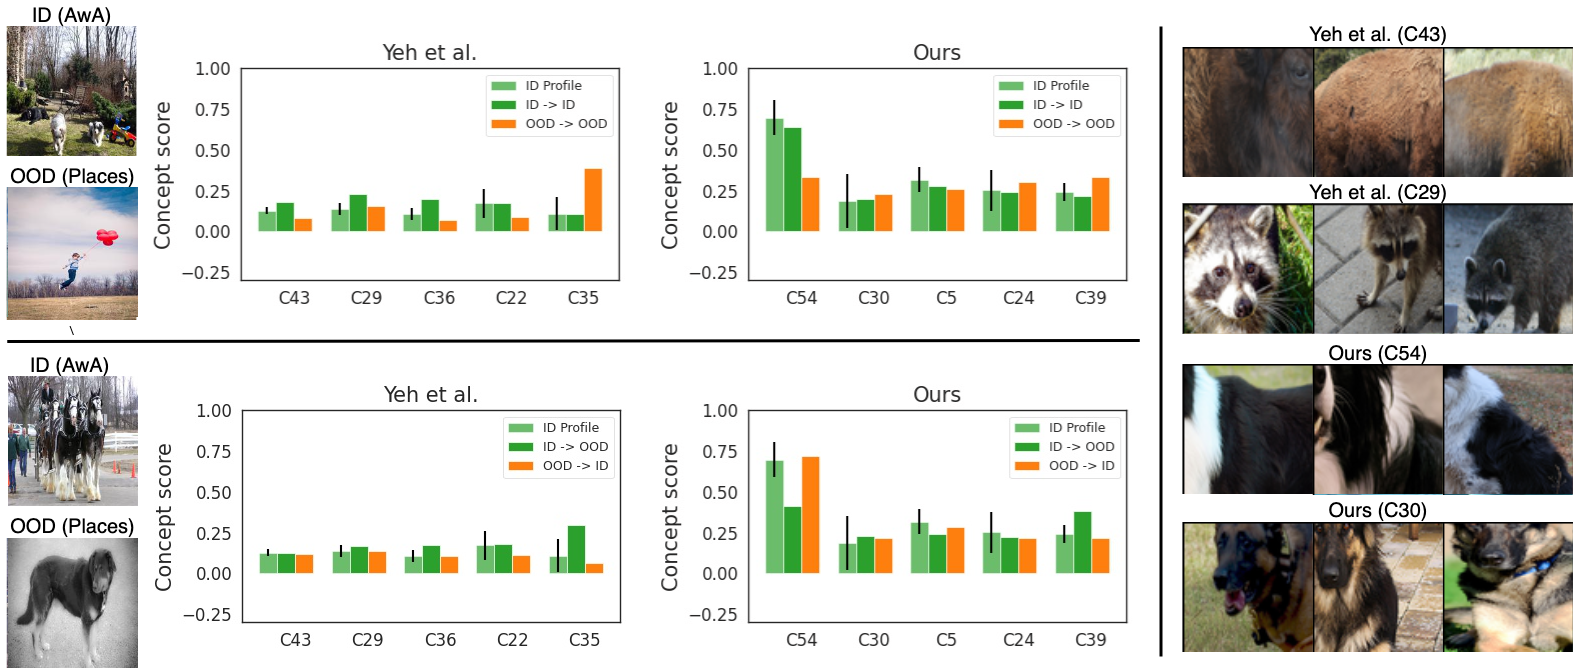
\includegraphics[width=0.9\textwidth]{figures/energy-collie.png}
\caption{\small \textbf{Concept-based explanations for the Energy OOD detector using concepts learned by \citet{yeh2020completeness} vs. ours ($\lambda_\textrm{mse} = 1, \lambda_\textrm{norm} = 0.1, \lambda_\textrm{sep} = 10$)}. Images are randomly selected from the AwA test set (ID) and \texttt{Places} (OOD), and all of them are predicted to the class ``Collie''.
The ID profile (light-green bar) shows the average concept-score pattern for ID images predicted as ``Collie''. 
The top two images correspond to correct detection, \ie ID detected as ID (dark-green bar) and OOD detected as OOD (orange bar).
Similarly, the bottom  two images correspond to incorrect detection.
The right sub-figure illustrates the top two concepts for the method of \citet{yeh2020completeness} and our method.
}
\label{fig:expl-energy-collie}
\vspace{-3mm}
\end{figure*}
\fi




\subsection{Concept-Based Explanations for OOD Detectors}
\label{sec:expt_concept_based_explanations}
% \mypara{Contribution of each concept to detection.}

\mypara{Finding the Key Concepts.}
Given a set of learned concepts, we address the question: {\em how much does each concept contribute to the detection results for inputs predicted to a particular class?}
To address this, we follow recent works that have adopted the Shapley value from Game theory literature~\citep{shapley1953value,fujimoto2006axiomatic} for scoring the importance of a feature subset towards the predictions of a model~\citep{chen2018shapley,lundberg2017shapley,sundararajan2020shapley}.
We propose to use our per-class detection completeness metric $\eta^{j}_{\bff, S}(\bfC)\,$ (Eqn. (\ref{equ: completeness-detection-perclass}) in Appendix \ref{sec:appendix-perclass-completeness}) as the characteristic function of the Shapley value. 
The modified Shapley value of a concept $\bfc_i \in \bfC$ with respect to the predicted class $j \in [L]$ is defined as
% \vspace{-3mm}
\begin{align}
    \label{equ: ConceptSHAP}
    \textrm{SHAP}(\eta^{j}_{\bff, S}, \bfc_i) ~:= \!\!\!\sum_{\bfC' \subseteq \bfC \setminus \{\bfc_i\}} \!\!\! \frac{ \eta^{j}_{\bff, S}\big( \bfC' \cup \{\bfc_i\} \big) ~-~ \eta^{j}_{\bff, S}(\bfC') }{ m\, \binom{m \,-\, 1}{|\bfC'|} },
\end{align}
where $\bfC'$ is a subset of $\bfC$ excluding concept $\bfc_i$.
% A high Shapley value represents the average marginal contribution of $\bfc_i$ across all possible coalitions with all classes considered.
This Shapley importance score captures the average marginal contribution of concept $\bfc_i$ towards explaining the decisions of the OOD detector for inputs predicted into class $j$.
% To do so, we simply modify our detection completeness definition (Def. (\ref{def:completeness_detec})) into a per-class variant by considering data predicted into a specific class $j$.
% Also, $b_r = 0.5$ is the AUROC of a random detector.
% Note that for numerator we use predicted label -- don't have labels for OOD data. 
% Accordingly, we use SHAP($\eta^{j}_{\bff, S}(\bfC)$) to denote the Shapley score specific to class $j$.
% where $\eta^{}_{\bff, S}(\bfC)$ is replaced in Eqn. (\ref{equ: completeness-detection-perclass}).

In the rest of the section, we demonstrate how the concepts ranked by the above Shapley importance score can serve as a useful tool for interpreting the OOD detector.


\mypara{Explaining Detection Errors.}
% Eventually, we interpret the behavior of the given OOD detector by plotting the concept score patterns with respect to the concepts ranked by the above Shapley importance score.
Given an OOD detector of interest, we collect inputs that are correctly detected as ID, and average their concept scores (which corresponds to the \textit{ID profile} in Fig.~\ref{fig:expl-energy-collie}).
The ID profile quantifies how much each concept matters for the normal ID inputs.
Given a test input, either correctly or incorrectly detected, the user could examine how similar or different this input is with respect to the ID concept profile.
Fig.~\ref{fig:expl-energy-collie} illustrates our explanations of the Energy OOD detector's decisions.
By visualizing the concepts (see Fig.~\ref{fig:collie-concepts}), we observe that for the predicted class \textit{Collie}, ``furry dog skin'' (C54) and ``oval dog face'' (C30) are the key concepts to capture the detector's outputs to distinguish ID images from OOD images.
% given correctly-detected inputs (ID\,/\,OOD input detected as ID\,/\,OOD; first row of figure), and incorrectly-detected inputs (ID\,/\,OOD input detected as OOD\,/\,ID; second row of figure).
We also observe that the OOD detector predicts an input as ID when the concept scores show a similar pattern to the ID profile, or predicts an input as OOD when the concept-score pattern is far from the ID profile.
For instance, our analysis shows that the bottom input in Fig.~\ref{fig:collie-wrong} is an OOD image from \texttt{Places} dataset but detected as ID (false positive) since its score for ``furry dog skin'' is as high as the usual ID Collie images (which is true in the image). 
Explaining detection results is crucial for encouraging the adoption of OOD detectors in various decision-making processes.
Our example here suggests that certain errors of an OOD detector can be understandable mistakes, which require further reasoning, rather than discarding the model based only on aggregate performance  metrics.
% Thus, we conclude this to be an understandable mistake by the OOD detector.
Additional examples of our concept-based explanations are given in Appendix~\ref{app:more-expl}.

\mypara{Comparison of Explanations by~\citeauthor{yeh2020completeness} and Ours.}
Lastly, we provide qualitative evidence supporting our argument that: concepts good for the classifier are not necessarily good for the OOD detector.
In Fig.~\ref{fig:expl-energy-collie}, given an Energy detector and ID/OOD inputs, we present explanations using  concepts learned by \citet{yeh2020completeness} vs. our method.
We observe that~\citet{yeh2020completeness} fails to generate visually-distinguishable explanations between detected-ID and detected-OOD inputs.
The separation between the dark-green bars and the orange bars in Fig.~\ref{fig:collie-correct} and Fig.~\ref{fig:collie-wrong} becomes more visible in our explanations, which enables more intuitive interpretation for human users (this reflects our design goal of concept separability).
It is also noteworthy that in Fig.~\ref{fig:collie-concepts}, our concepts that are most important to distinguish ID Collie from OOD Collie (\ie C54 and C30) are more specific and finer-grained characteristics of Collie, while \citet{yeh2020completeness} finds concepts that are vaguely similar to the features of a dog, but rather generic (\ie C43 and C29).
This is the reason we require more number of concepts to achieve high detection completeness and concept separability, compared to solely considering the classification completeness~\footnote{In Fig.~\ref{fig:expl-energy-collie}, after concept learning with $m = 100$ and duplicate removal, we found 44 non-redundant concepts for ~\citet{yeh2020completeness}, and 100 distinct concepts for ours.}.
% \jihye{@others: may add one more closing/concluding statement?}


% \subsection{Bootstrapping explanations for better OOD detection}
\subsection{Explanations For Better OOD Detection.}
Our work makes the first effort to reason about the different failure modes of OOD detectors through explanations, rather than just observing aggregated performance metrics (e.g., AUROC or AUPRC).
Naturally, the next step would be to utilize such reasoning to modify and improve the OOD detector. 
% While leaving the development of concept-based explanations as actionable guidelines for better OOD detection as a future work, here we provide a scenario where our explanations can provide direct utility.
We leave the development of concept-based explanations as actionable guidelines for better OOD detection as future work, and describe here a scenario where our explanations can provide direct utility.

We posit that our explanations can provide effective feedback when the failure of the OOD detector originates from misbehavior of the paired classifier, which we confirm to be the most common failure mode of OOD detectors. 
For instance, consider the top image in Fig.~\ref{fig:collie-wrong} as our input. Its true label is ``Horse'', but the classifier predicted it to class ``Collie''. Obviously, the horse image has a different concept-activation pattern from the normal ID Collie profile (compare the dark-green bars with the ID profile of ours in Fig.~\ref{fig:collie-wrong}). 
To remove such failure cases, the practitioner could identify the key concepts for the prediction of class ``Horse'' and compare the concept pattern of the input to the normal ID ``Horse'' profile. It is noteworthy that we can use the same set of concepts here, since our concept-learning objective finds concepts that can effectively explain \textit{both} the classifier and OOD detector. Indeed, we observe that the key concepts for the class ``Horse'' are ``round brown body'' and ``brown oval face of horse'', while the given input is an outlier relative to these concepts. 
Hence, the practitioner could consider diversifying the training set in the ID ``Horse'' class to include more examples of horses (\eg with black and white hair).

\iffalse

Based on this concept importance metric, we can interpret the misbehavior of the given OOD detector.
Fig. \ref{fig:expl_dolphin} shows the averaged concept scores of top-10 important concepts for Energy detector between correctly detected-ID and -OOD inputs that are predicted to class ''Dolphin'' (namely, correct profiles).
Given a random ID input that is mis-detected into OOD by the OOD detector, we observe that its concept scores rather follow the detected-OOD profiles (or vice-versa, for OOD input mis-detected into ID); specifically, unusually low score for C1 (blue, wavy surface of the sea) and high score for C14~\footnote{We could not visualize C14 as there is no receptive fields with correlation to $\bfc_{14}$ greater than $0.85$, which confirms the trade-off between concept separability and human understandability, as discussed in Appendix \ref{sec:appendix-concept-learning-ablation}}, and it would look reasonable for the OOD detector to think the ID input with such OOD-like characteristics to be OOD. 
Such inspection of the OOD detector's mistakes could assist the practitioner in examining whether it was a reasonable mistake even for humans, or whether the OOD detector is simply unreliable. See Appendix \ref{sec:appendix-shapleys} for more examples of explanations.

More examples can be found in Appendix.
we present the top-ranked concepts along with the visualized examples that are nearest to the corresponding concept vector in Fig. \ref{fig:shap_buffalo}.
For the baseline method \citep{yeh2020completeness} (denoted ``baseline'' in Fig. \ref{fig:shap_buffalo}), the learned concepts are solely intended for reconstructing the behavior of the classifier. 
In this case, we observe from Fig. \ref{fig:shap_buffalo} that 
% a common set of concepts (\ie concepts 32, 10, and 47) are selected for interpreting both the classifier and OOD detector.
interpretation of both the classifier and OOD detector depends on a common set of concepts (\ie concepts 32, 10, and 47).
On the other hand, the concepts learned by our method focus on reconstructing the behavior of both the OOD detector and the classifier. In this case, we observe from Fig. \ref{fig:shap_buffalo} that a distinct set of important concepts are selected for classification and OOD detection.
We also observe that our method requires more concepts in order to address the decisions of both the classifier and OOD detector.
For instance, the number of concepts obtained by our method and the baseline are 78 and 53 (respectively), out of a total 100 concepts~\footnote{After removing redundant concepts for which the inner-product between the corresponding concept vector and any of the remaining concept vectors is larger than $0.95$.}.
More examples of concepts with high-ranking Shapley scores can be found in Appendix \ref{sec:appendix-explanation}.
We further investigate the attribution of such top-ranked concepts via counterfactual analysis in Appendix \ref{sec:appendix-counterfactual}.

\fi

% \mypara{Separability and interpretatbility}
% \begin{figure*}
%   \centering
%   \begin{tabular}{cc}
%     \subfloat[\label{fig:mnist}][Sampling distribution is skewed consistently for a single class (i.e. class 0)]
%     {
%     \hspace{-5mm}
%     \includegraphics[width=.49\linewidth]{mnist_class_0}} 
%     ~&~
%     \subfloat[\label{fig:asd}][Sampling distribution is skewed for the classes in turn (i.e. class 0, 1, 2, ...)]
%     {\includegraphics[width=.49\linewidth]{mnist_class_all}}
%   \end{tabular}
%   \caption{Accuracy vs training time-step in MNIST}
% \label{fig:mnist_results}
% \end{figure*}
